\section{Client-server view (UML Component diagram)}\label{sec:client-server}
In Figure \ref{fig:cc-context}, we present a context diagram of the client-server view, detailing the external communication to and from the system. The entry points to the system are the (mostly automated) external version of raw data submission. The Customer Organisation and/or Social Secretary can submit Raw Data Batches via the specified protocols supported by the eDocs system.
The other entry point being the \texttt{UIfacade}, which is contacted by User Software for User Interface Actions, e.g. a management dashboard for the Customer Administrator (one or more per Organisation) to query for job statuses, or a log-in system for recipients to log in to the PDS.
The exit points of the system are more versatile. There is one closely related to the UI Actions, where parts of the system respond to queries by directly supplying information to the user sessions, which in turn are individual (dedicated) intermediaries for instances of the client software. This bypasses the \texttt{UIFacade} as a bottleneck.
The \texttt{SubmissionSubsystem} queries an \texttt{External Information Broker} when verifying the meta-data of Raw Data Batches and Entries as specified in \emph{UC3}.
The \texttt{BillingSubsystem} contacts the \texttt{Billing System} (external of the actual eDocs system) used by the eDocs Company periodically to bill users of eDocs.
The \texttt{CommunicationSubsystem} submits composed e-mails to an \texttt{External Email Provider} for delivery. This functionality is used for reporting errors in the system to the eDocs admin, various notifications to CO admins, delivery of documents etc.
There are two other external communication mechanisms for document delivery, namely the \texttt{Zoomit} service's \texttt{Document Delivery} interface and the \texttt{Print \& Postal Service}'s one. These are both directly used by the delivery subsystem, in contrast to document delivery by e-mail, which passes through the \texttt{CommunicationSubsystem}, as explained earlier.

\begin{figure}[!htp]
    \centering
    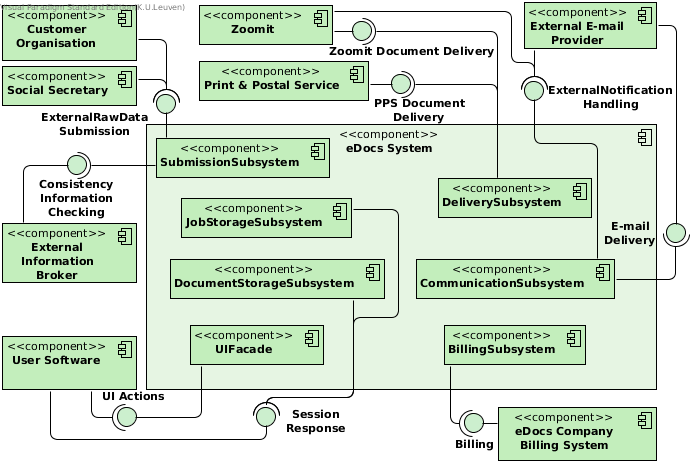
\includegraphics[width=\textwidth]{figures/Context Diagram 1.png}
    %\missingfigure[figwidth=0.8\textwidth]{Context diagram of the client-server view.}
    \caption{Context diagram for the client-server view.}\label{fig:cc-context}
\end{figure}

The primary diagram and accompanying explanation.

\begin{figure}[!htp]
    \centering
    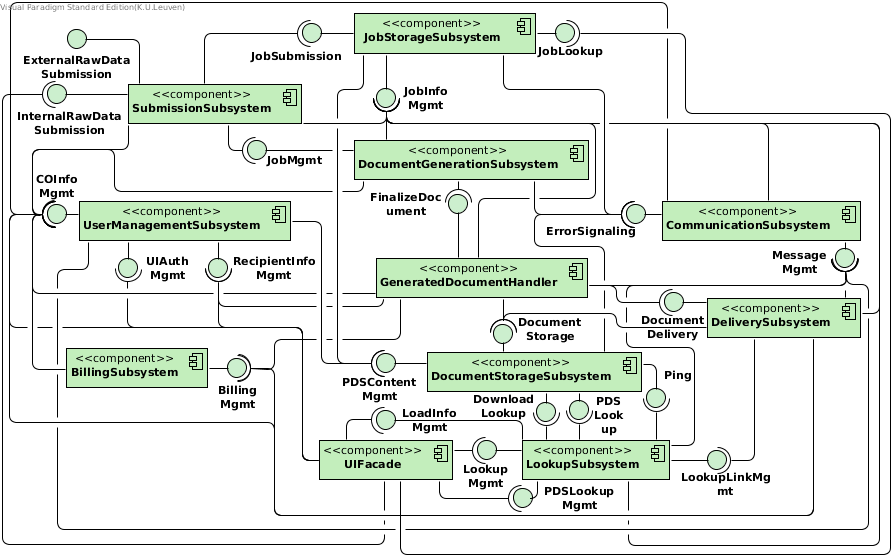
\includegraphics[width=\textwidth]{figures/Subsystem Diagram.png}
    %\missingfigure[figwidth=0.8\textwidth]{Primary diagram of the client-server view.}
    \caption{Primary component-and-connector view of the proposed architecture.}\label{fig:cs-primary}
\end{figure}

\subsection{Main architectural decisions}
Discuss your architectural decisions for the most important requirements in
more detail using the components of the client-server view.
Pay attention to the solutions that you employed and the alternatives that you
considered.
The explanation here must be self-contained and complete.
Imagine you had to describe how the architecture supports the core
functionality to someone that is looking at the client-server view only.
Hide unnecessary details (these should be shown in the decomposition view).

\subsubsection{ReqX\@: requirement name}
Describe the design choices related to \emph{ReqX} together with the rationale
of why these choices where made.

\subsubsection*{Alternatives considered}
\paragraph{Alternative(s) for choice 1} Explain what alternative(s) you
considered for this design choice and why they where not selected.
